
%W5100

Η χρήση του ολοκληρωμένου επιλέγεται να γίνει δια μέσω της πλακέτας WIZ811MJ της
ίδιας εταιρείας. Οι λόγοι είναι ότι επιλύει τη διασύνδεση του ολοκληρωμένου με
συνδετήρα RJ-45 (απαραίτητος για την ανταλλαγή δεδομένων μεταξύ W5100 και
δικτύου), ταλαντωτή και διάφορα άλλα ηλεκτρονικά στοιχεία. Από τους 80,
συνολικά, ακροδέκτες του W5100, το WIZ811MJ διαθέτει μόλις 40, οι οποίοι είναι
αυτοί που προορίζονται για τη διασύνδεση με μικροελεγκτή. Όλοι οι υπόλοιποι
συμμετέχουν σε εσωτερικές συνδέσεις της πλακέτας.

Ένα παράδειγμα σχετικά με το τελευταίο, το W5100 διαθέτει έναν ακροδέκτη για το
χειρισμό του ολοκληρωμένου ως Slave σε δίαυλο SPI, το \nbar{SCS}
(\textenglish{SPI Chip-Select}) \parencite[9]{wiz11:w5100}. Ωστόσο, διαθέτει και
έναν επιπρόσθετο ακροδέκτη, τον SEN (\textenglish{SPI Enable}), για την
ενεργοποίηση των υποσυστημάτων του ολοκληρωμένου για λειτουργία σε SPI
\parencite[8]{wiz11:w5100}. Το WIZ811MJ παρέχει ακροδέκτη μόνο για το \nbar{SCS}
ενώ διαθέτει κατάλληλη διάταξη ώστε η αλλαγή της τιμής του να προκαλεί το
αναμενόμενο σήμα στο SEN, αυτομάτως \parencite[7]{wiz13:811mj}.

Επιπλέον σημαντικό χαρακτηριστικό είναι ότι η πλακέτα παρέχει ακροδέκτες
συμβατούς με πρωτότυπες κάρτες (\textenglish{breadboard}) που χρησιμοποιεί η
υλοποίηση, εν αντιθέσει με το W5100 το οποίο είναι SMD
(\textenglish{Surface-Mount Device}) και απαιτεί συγκόλληση
\parencite[6,12]{wiz13:811mj}.


%\subsection{Επικοινωνία με μικροελεγκτή}
\subsection{Διασύνδεση με μικροελεγκτή}

Το W5100 υποστηρίζει τρεις τρόπους για την επικοινωνία με το μικροελεγκτή· άμεση
ή έμμεση προσπέλαση ή, μέσω πρωτοκόλλου SPI \parencite[59]{wiz11:w5100}. Οι δύο
πρώτες μέθοδοι χρησιμοποιούν διαύλους διεύθυνσης και δεδομένων απαιτώντας πολλά
σημεία σύνδεσης με το μικροελεγκτή· για την ακρίβεια, 3 γραμμές ελέγχου
(\textenglish{Chip-Select, Read, Write}), 8 γραμμές για το δίαυλο δεδομένων,
και, 15 ή 2 γραμμές διεύθυνσης για άμεση ή έμμεση προσπέλαση, αντίστοιχα. Στην
περίπτωση του SPI απαιτούνται πολύ λιγότερες (μόλις 4) και αυτός είναι ο λόγος
που προτιμάται για τη διασύνδεση του με το μικροελεγκτή, δεδομένου του
περιορισμένου αριθμού ακροδεκτών του.
Σαφώς, το μειονέκτημα χρήσης SPI -- ενός σειριακού
πρωτοκόλλου επικοινωνίας -- είναι ότι επιτυγχάνεται πολύ μικρότερος ρυθμός
ανταλλαγής δεδομένων από ότι στην περίπτωση των άλλων δύο, κάτι που, τελικά,
επηρεάζει το χρόνο απόκρισης στα εισερχόμενα αιτήματα. Ωστόσο, κρίνεται ότι για
τις ανάγκες της υλοποίησης, αυτός ο περιορισμός είναι αμελητέος σε σχέση με την
εξοικονόμηση ακροδεκτών που επιφέρει η χρήση SPI.

\begin{figure}
    \caption{Πλακέτα WIZ811MJ και διάταξη των ακροδεκτών του W5100.
    \label{fig:net:811mj-pins}}
    \begin{center}
    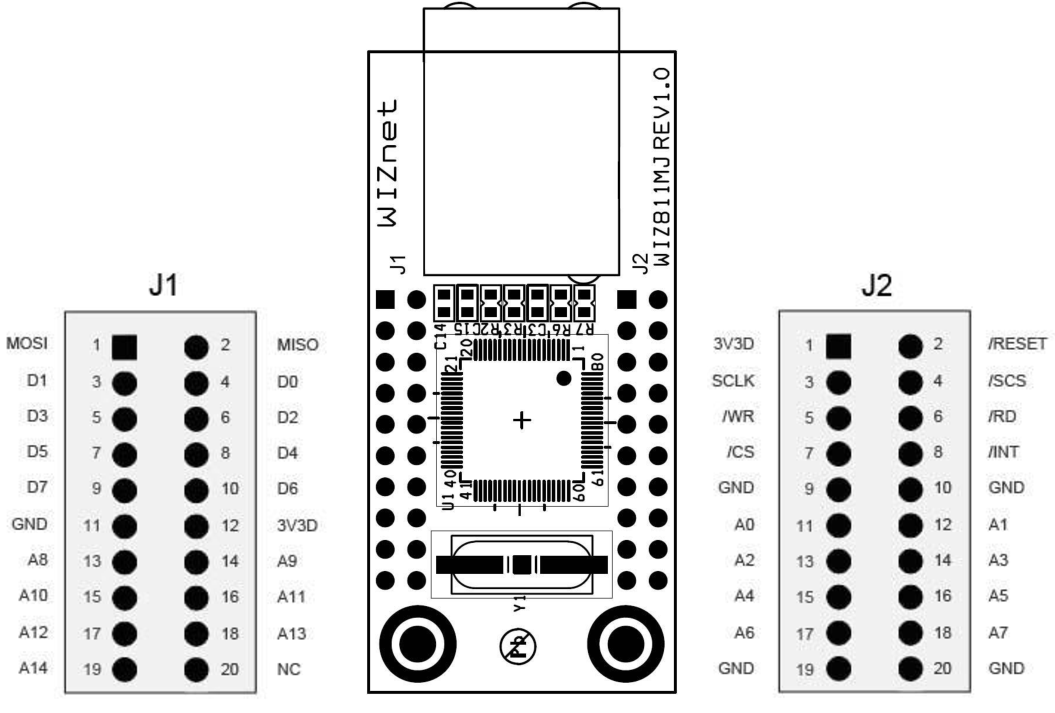
\includegraphics[width=0.9\textwidth]{network_811mj_pin-layout}
    \end{center}
    \fullcite[6]{wiz13:811mj:pins}
\end{figure}


\subsubsection{Συνδεσμολογία}

Το σχήμα \ref{fig:net:811mj-pins} παρουσιάζει την πλακέτα WIZ811MJ και, σε
μεγέθυνση, την ονομασία των ακροδεκτών της. Από τους ακροδέκτες J1, ιδιαίτερου
ενδιαφέροντος είναι οι 1 (MOSI), 2 (MISO) και 12 (3V3D) εκ των οποίων οι δύο
πρώτοι χρησιμοποιούνται για την μετάδοση των bit του \textenglish{Master} και
του ενεργού \textenglish{Slave} του διαύλου SPI, αντίστοιχα, ενώ ο τελευταίος,
για την τροφοδοσία της πλακέτας με τάση 3.3V. Οι υπόλοιποι, με εξαίρεση τον 20
(\textenglish{Not Connected}), συνδέονται με την τάση αναφοράς, δεδομένου ότι
όλοι, με εξαίρεση τον ακροδέκτη 11 (GND), χρησιμοποιούνται μόνο στην περίπτωση
άμεσης ή έμμεσης προσπέλασης.

Από τους ακροδέκτες J2, ο 1 (3V3D) χρησιμοποιείται για τροφοδοσία 3.3V ενώ οι
9, 10, 19 και 20 (GND) συνδέονται με την τάση αναφοράς. Οι 3 (SCLK) και
(\nbar{SCS}) αποτελούν μέρος του διαύλου SPI για τη μεταφορά του ρολογιού από
το \textenglish{Master} και την ενεργοποίηση του W5100 ως \textenglish{Slave}.
Σύμφωνα με το εγχειρίδιο της \textcite[8]{wiz13:811mj}, ο ακροδέκτης 2
(\nbar{RESET}) προκαλεί την αρχικοποίηση όλων των καταχωρητών του W5100 στις
προεπιλεγμένες τους τιμές και κρίνεται ότι αρκεί να συνδεθεί με το αντίστοιχο
σήμα του μικροελεγκτή ώστε η αρχικοποίηση του W5100 να πραγματοποιείται μαζί
με του μικροελεγκτή.

Οι ακροδέκτες 5 (\nbar{WR}), 6 (\nbar{RD}) και 7 (\nbar{CS}) χρησιμοποιούνται
στην περίπτωση επικοινωνίας μέσω άμεσης ή έμμεσης προσπέλασης και όχι σε SPI
\parencite[8]{wiz11:w5100}. Ωστόσο, επειδή τα σήματα είναι
\textenglish{active low}, τίθενται σε μόνιμο λογικό 1 (3.3V), μέσω αντιστάτη,
ώστε να είναι λογικά ανενεργά.

Μέσω του ακροδέκτη 8 (\nbar{INT}), και εφόσον έχει διευθετηθεί ακολούθως, το
W5100 αναγγέλλει την επιθυμία του για επικοινωνία με το μικροελεγκτή (για
παράδειγμα, επειδή έχουν καταφθάσει δεδομένα). Σε αντίθετη περίπτωση, ο
μικροελεγκτής είναι υποχρεωμένος να εξετάζει από μόνος του το ενδεχόμενο για
επικοινωνία (\textenglish{polling}). Για την υλοποίηση, κρίνεται αξιόλογη η
χρήση των διακοπών. Περισσότερες λεπτομέρειες παρέχονται στην
\nameref{ssubsec:network:ir_imr} (σ. \pageref{ssubsec:network:ir_imr}).

Για λόγους που έχουν αναφερθεί, όλοι οι υπόλοιποι ακροδέκτες συνδέονται με την
τάση αναφοράς.

\begin{figure}
    \caption{Διασύνδεση μικροελεγκτή και W5100.
    \label{fig:network:spi_reset_int}}
    \begin{center}
    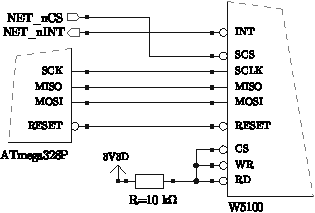
\includegraphics{network_schem_spi_reset_int}
    \end{center}
\end{figure}

Στο σχήμα \ref{fig:network:spi_reset_int} εμφανίζεται η συνδεσμολογία του
μικροελεγκτή με τους ακροδέκτες του W5100 (δια μέσω της πλακέτα WIZ811MJ).
Αξίζει να σημειωθεί ότι, παρόλο που το W5100 λειτουργεί με τάση έως και 3.6V,
ανέχεται τάση στα σήματα εισόδου έως και 5.5V (\textenglish{5V tolerant})
\parencite[64]{wiz11:w5100}. Το χαρακτηριστικό αυτό είναι ιδιαίτερα σημαντικό
επειδή καθιστά δυνατή τη διασύνδεσή του με το μικροελεγκτή χωρίς να απαιτούνται
επιπρόσθετα ενδιάμεσα κυκλώματα για λογικό μετασχηματισμό. %\nref{}


\subsubsection{Πρωτόκολλο επικοινωνίας}

Το πρότυπο διαύλου επικοινωνίας SPI καθορίζει τα ηλεκτρικά χαρακτηριστικά για
την επίτευξη αμφίδρομης ταυτόχρονης bit-προς-bit ζεύξης επικοινωνίας μεταξύ
Master και Slave διατάξεων.
% \nref: Ανάλυση SPI
Σε αυτήν την υποδομή στηρίζεται το πρωτόκολλο του W5100, το οποίο με απλές
εγγραφές και αναγνώσεις των διευθύνσεων μνήμης επιτυγχάνει την επιθυμητή
συμπεριφορά του W5100.

Στο σχήμα \ref{fig:network:w5100-command-format} εμφανίζεται η δομή των εντολών,
οι οποίες συνίστανται από ένα Byte κωδικού (\te{op-code}), δύο Byte διεύθυνσης
(\te{address-H} και \te{address-L}) και ένα Byte φορτίου (\te{payload}). Ο
κωδικός αποστέλλεται πρώτος και προσδιορίζει εάν πρόκειται να εκτελεστεί εγγραφή
(\verb~0xF0~) ή ανάγνωση (\verb~0x0F~) στη διεύθυνση μνήμης που καθορίζεται από
τα επόμενα δύο Byte (με το πλέον σημαντικό Byte να αποστέλλεται πρώτο)
\parencite[61]{wiz11:w5100}.
Στην περίπτωση όπου γίνεται ανάγνωση, η τιμή του φορτίου είναι αδιάφορη καθώς τα
8bit φορτίου αποστέλλονται ώστε να δοθεί η ευκαιρία στο W5100 να επιστρέψει τα
περιεχόμενα της αντίστοιχης διεύθυνσης (\te{dummy data}).

\begin{figure}
    \caption{Δομή εντολής W5100 μέσω SPI.
    \label{fig:network:w5100-command-format}}
    \begin{center}\begin{tabu} spread 0pt {|*4{X[1,c]|}}

    \hline
    op-code & address-H & address-L & payload \\
    \hline

    \end{tabu}\end{center}
\end{figure}

Πλέον, είναι εύληπτη η επιβάρυνση που επιφέρει η χρήση SPI στη συγκεκριμένη
περίπτωση καθώς μεταφέρονται 32bit για, μόλις, 8bit πραγματικού φορτίου.

Επιπλέον, σύμφωνα με τις προδιαγραφές χρονισμού της \textcite[66]{wiz11:w5100},
η μέγιστη υποστηριζόμενη συχνότητα ρολογιού υπολογίζεται περίπου στα 14MHz. Με
τις τρέχουσες επιλογές της υλοποίησης, το ρολόι συστήματος ανέρχεται στα 4MHz
με αποτέλεσμα η μέγιστη συχνότητα ρολογιού SPI που δύναται να παραχθεί από το
μικροελεγκτή να είναι, σύμφωνα με το εγχειρίδιο της
\textcite[179--180]{atmel13}, τα 2MHz· κατά πολύ χαμηλότερη από το προαναφερθέν
μέγιστο όριο.
% \nref: Συχνότητα ρολογιού συστήματος


\subsection{Διευθέτηση W5100}

Οι καταχωρητές του W5100 χωρίζονται σε δύο κύριες ομάδες· τους καταχωρητές
γενικών ρυθμίσεων (ή κοινοί καταχωρητές) και τους καταχωρητές Socket. Οι κοινοί
καταχωρητές επηρεάζουν τη συμπεριφορά του W5100 συνολικά ή προσδιορίζουν κάποια
χαρακτηριστικά όλων των Socket, ενώ οι καταχωρητές Socket είναι υπεύθυνοι για
τη λειτουργία καθενός εκ των τεσσάρων Socket του ολοκληρωμένου.

Όλοι οι καταχωρητές αντιστοιχίζονται μία διεύθυνση, ενώ υπάρχουν καταχωρητές
περισσοτέρων του ενός byte. Η πρόσβαση σε αυτούς τους καταχωρητές, είτε
πρόκειται για ανάγνωση είτε για εγγραφή, γίνεται από τη χαμηλότερη προς την
υψηλότερη διεύθυνση με \te{Big Endian} διάταξη των byte
\parencite[32--33,35]{wiz11:w5100}.

Οι κοινοί καταχωρητές τίθενται μόνο μία φορά, κατά την εκκίνηση της συσκευής,
και, οι ορισμένοι, κατόπιν εισερχόμενων αιτημάτων (για παράδειγμα, αλλαγή
διεύθυνσης IP). Σε αντίθεση, η πρόσβαση στους καταχωρητές Socket, οι οποίοι
χρησιμοποιούνται για το χειρισμό κάθε Socket, είναι πιο συχνή.


\subsubsection{Καταχωρητές διευθύνσεων και μάσκας υποδικτύου}
\label{ssubsec:network:addr-registers}

Σε αυτήν την κατηγορία συγκαταλέγονται καταχωρητές που ρυθμίζουν τη διεπαφή για
τη σύνδεση με το δίκτυο μέσω των GAR (\te{Gateway Address Register}),
SUBR (\te{Subnet Mask Register}), SHAR (\te{Source Hardware Address Register})
και SIPR (\te{Source IP Address Register}) \parencite[20]{wiz11:w5100}. Η αλλαγή
της τιμής κάποιου, έχει άμεση εφαρμογή στη διεπαφή, γεγονός που λαμβάνεται υπόψη
σε σχετικά εισερχόμενα αιτήματα ώστε να δίνεται απόκριση με τις τρέχουσες
ρυθμίσεις της διεπαφής πριν την ενημέρωσή τους.
% \nref: stored in back-up memory.


\subsubsection{Μέγεθος μνήμης ανά Socket}
\label{ssubsec:network:rmsr_tmsr}

Το W5100 υποστηρίζει μέχρι τέσσερα, ταυτόχρονα, ενεργά Socket καθένα από τα
οποία αποδίδεται ένα μέρος μνήμης από τα συνολικά διαθέσιμα 8KiB για κάθε
κατεύθυνση κίνησης δεδομένων, ανεξάρτητου μεγέθους το καθένα. Οι καταχωρητές
RMSR (\te{RX Memory Size Register}) και TMSR (\te{TX Memory Size Register})
καθορίζουν την προσωρινή μνήμη που αφιερώνεται σε κάθε Socket μεταξύ 1, 2, 4 ή 8
KiB. Σαφώς, πρέπει να δίνεται προσοχή ώστε ο ανατεθειμένος χώρος στα Socket
να μην ξεπερνάει τα 8KiB καθώς, σε αυτήν την περίπτωση, ορισμένα Socket θα
εργάζονται σε κοινές θέσεις στη μνήμη, με ότι επακόλουθα μπορεί αυτό να
επιφέρει.

\begin{figure}
    \caption{Καταχωρητές μεγέθους, RMSR και TMSR.\label{fig:network:rmsr_tmsr}}
    \begin{center}\begin{tabu} spread 0pt {|*8{X[-1,c]|}}

    \hline\rowfont\bfseries
    \multicolumn2{|c}{Socket 3}     &
    \multicolumn2{|c}{Socket 2}     &
    \multicolumn2{|c}{Socket 1}     &
    \multicolumn2{|c|}{Socket 0}   \\

    \hline

    S1  &  S0  &  S1  &  S0  &  S1  &  S0  &  S1  &  S0                       \\
    \hline
    \end{tabu}\end{center}

    Το μέγεθος κάθε Socket καθορίζεται από την τιμή $2^{\text{S1:0}}$.
\end{figure}

Το σχήμα \ref{fig:network:rmsr_tmsr} παρουσιάζει τη σημασιολογία των bit των
δύο αυτών καταχωρητών. Παρατηρείται ότι το μέγεθος της μνήμης κάθε Socket
ρυθμίζεται από δύο, μόνο, bit.
Η υλοποίηση χρησιμοποιεί μόνο ένα Socket με σκοπό τη λήψη και απόκριση αιτημάτων
HTTP. Για το λόγο αυτό οι RMSR και TMSR ρυθμίζονται ώστε να αποδίδονται 8KiB
τόσο για την εισερχόμενη όσο και για την εξερχόμενη προσωρινή μνήμη αποθήκευσης
του Socket 0. Οι ρυθμίσεις του Socket ολοκληρώνονται στην παράγραφο
\nameref{ssubsec:network:port_mr} (σ. \pageref{ssubsec:network:port_mr}).


\subsubsection{Κατάσταση και διακοπές}
\label{ssubsec:network:ir_imr}

Δύο τελευταίοι καταχωρητές που εξετάζονται είναι οι IR(\te{Interrupt Register})
και IMR (\te{Interrupt Mask Register}), οι οποίοι καθορίζουν την κατάσταση
του W5100 και την αναγγελία διακοπών, αντιστοίχως· τα bit του καταχωρητή IR --
μόνο για ανάγνωση -- τίθενται σε κάθε περίπτωση που το απαιτεί, ενώ διακοπή
(μέσω του ακροδέκτη \nbar{INT}) προκαλείται μόνο όταν τίθενται bit του IR των
οποίων το αντίστοιχο bit του IMR έχει, επίσης, τεθεί
\parencite[21--22]{wiz11:w5100}. Με αυτόν τον τρόπο, αναγγέλλονται μόνο οι
διακοπές που ενδιαφέρουν. Επιπλέον, ο μικροελεγκτής εξετάζοντας τον IR μπορεί,
ανά πάσα στιγμή, να αποφασίσει εάν το W5100 χρειάζεται την προσοχή του.

Τα bit των καταχωρητών IR και IMR παρουσιάζονται στο σχήμα
\ref{fig:network:ir_imr}. Από τα συνολικά 7 διαθέσιμα bit, μόνο το S0\_INT που
ειδοποιεί για αλλαγή της κατάστασης του  -- μοναδικού ενεργού -- Socket 0 έχει
ενδιαφέρον για την υλοποίηση και για το λόγο αυτό, τίθεται σε λογικό 1 στον
καταχωρητή IMR. Για λεπτομέρειες σχετικά με τη φύση της διακοπής είναι
απαραίτητη η εξέταση του αφιερωμένου καταχωρητή κάθε Socket.
% \nref: Sn_IR.

\begin{figure}
    \caption{Καταχωρητές κατάστασης και διακοπών, IR και IMR.
    \label{fig:network:ir_imr}}
    \begin{center}\begin{tabu} spread 0pt {|*8{X[-1,C]|}}

    \hline
    \rowfont\bfseries
           7 &       6 &     5 &  4 &       3 &       2 &       1 &       0   \\
    \hline
    CONFLICT & UNREACH & PPPoE & -- & S3\_INT & S2\_INT & S1\_INT & S0\_INT   \\
    \hline
    \end{tabu}\end{center}
\end{figure}

Ένα σημαντικό σημείο είναι ότι το σήμα του ακροδέκτη \nbar{INT} τίθεται και
παραμένει σε λογικό 0 μέχρι να διευθετηθούν όλα τα ενεργοποιημένα, για διακοπή,
bit του IR. Το χαρακτηριστικό αυτό χρησιμοποιείται, στο πλαίσιο της υλοποίησης,
σε συνδυασμό με έναν από τους ακροδέκτες INTn του μικροελεγκτή, ώστε η ρουτίνα
εξυπηρέτησης διακοπής να εκτελείται σε σήμα λογικού 0, και όχι σε παρυφή. Η
διευθέτηση αυτή έχει το πλεονέκτημα ότι ακόμα και εάν ο μικροελεγκτής έχει τεθεί
σε κατάσταση χαμηλής κατανάλωσης (\te{Power-down}), είναι βέβαιο ότι το σήμα
στον \nbar{INT} θα προκαλέσει, εκτός από αφύπνιση της CPU, και την εκτέλεση της
αντίστοιχης ρουτίνας εξυπηρέτησης. Όπως αναφέρεται στο εγχειρίδιο της
\textcite[71]{atmel13}, το τελευταίο είναι κάτι που πρέπει να ληφθεί υπόψη όταν
χρησιμοποιούνται παρυφές για την αφύπνιση καθώς, εάν η διάρκειά τους είναι
σύντομη, παρότι η CPU θα αφυπνιστεί, ενδέχεται να μην αναγνωριστεί η διακοπή.
Έτσι, εξαλείφεται αυτό το ενδεχόμενο.
%\nref : Wake-up from power-down mode.


\subsubsection{Θύρα και πρωτόκολλο Socket}
\label{ssubsec:network:port_mr}

Ένα Socket για να λειτουργήσει χρειάζεται, εκτός από διεύθυνση IP, αριθμό θύρας.
Η διεύθυνση που χρησιμοποιούν όλα τα ενεργά Socket του W5100 είναι αυτή που
καθορίζεται από τους
\nameref{ssubsec:network:addr-registers}
(σ. \pageref{ssubsec:network:addr-registers}).
Ωστόσο, ο αριθμός θύρας, προσδιορίζεται για κάθε Socket ξεχωριστά από τον
καταχωρητή Sn\_PORT.

Επιπλέον του αριθμού θύρας, το W5100 ρυθμίζεται με το πρωτόκολλο που
διεκπεραιώνει κάθε Socket. Η ρύθμιση γίνεται από τα τέσσερα τελευταία bit του
καταχωρητή Sn\_MR (\te{Socket n Mode Register}) \parencite[25--26]{wiz11:w5100}.
Στην περίπτωση της υλοποίησης, το μοναδικό ενεργό Socket προορίζεται για
παραλαβή αιτημάτων HTTP. Σύμφωνα με τους \textcite[13]{rfc2616}, το HTTP θεωρεί
ότι το υποκείμενο πρωτόκολλο παρέχει αξιόπιστη μεταφορά, και είθισται να είναι
το TCP, με αριθμό θύρας 80. Η υλοποίηση ακολουθεί αυτές τις καθιερωμένες
πρακτικές.


\subsubsection{Διαχείριση μνήμης Socket}
\label{ssubsec:network:rx-tx-buffer}

Στην παράγραφο
\nameref{ssubsec:network:rmsr_tmsr} (σ. \pageref{ssubsec:network:rmsr_tmsr})
περιγράφεται ο τρόπος απόδοσης μνήμης σε κάθε Socket για εισερχόμενα και
εξερχόμενα δεδομένα. Η λήψη και αποστολή των Byte αναλαμβάνεται, σαφώς, από το
W5100. Ωστόσο, το λογισμικό του μικροελεγκτή είναι υπεύθυνο για την ανάγνωση και
εγγραφή των κατάλληλων, κάθε φορά, διευθύνσεων της μνήμης του W5100.

\begin{figure}
    \caption{Μνήμη εισερχομένων για κάποιο Socket n.
    \label{fig:network:w5100-rx-buffer}}

    Όλα τα Socket αποδίδονται μέρος της κοινής μνήμης R\tsub{x}. Η μνήμη
    S\tsub{n} κάθε Socket συμπεριφέρεται ως δακτύλιος. Η γκρι περιοχή της
    εικόνας αντιπροσωπεύει δεδομένα.

    \begin{center}
    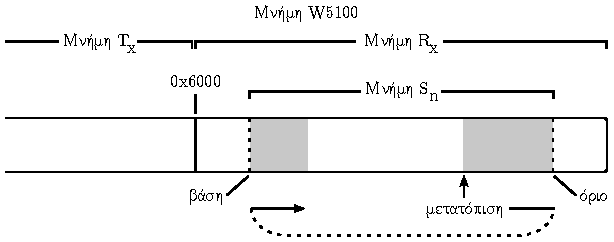
\includegraphics{network_w5100_rx-buffer}
    \end{center}
\end{figure}

Για την περίπτωση της μνήμης εισερχομένων, τα Socket διαθέτουν τους καταχωρητές
Sn\_RX\_RSR (\te{Socket n Rx Receive Size Register}) και
Sn\_RX\_RR (\te{Socket n Rx Read Register})· ο πρώτος αναγγέλλει το πλήθος, ενώ
από το δεύτερο είναι δυνατό να αναχθεί η διεύθυνση του πρώτου προς ανάγνωση
Byte, χωρίς, ωστόσο, να περιέχει ο ίδιος τη φυσική αυτή διεύθυνση
\parencite[35--36]{wiz11:w5100}. Σε σχέση με το τελευταίο, η αφιερωμένη μνήμη
κάθε Socket (Μνήμη S\tsub{n}, στο σχήμα \ref{fig:network:w5100-rx-buffer})
λειτουργεί ως δακτύλιος (κυκλική ουρά)· τα δεδομένα τοποθετούνται διαδοχικά από
τη βάση μέχρι το όριο (βλ. ίδιο σχήμα) και, μετά, πάλι από τη βάση.
Για κάθε νέο προστιθέμενο Byte, η τιμή του Sn\_RX\_RR αυξάνει κατά μία μονάδα,
ανεξαρτήτως εάν η αφιερωμένη μνήμη έχει γεμίσει ή όχι. Επομένως, η μετατόπιση
(\te{offset}) του πρώτου Byte (σε σχέση με τη βάση) είναι το υπόλοιπο της
διαίρεσης της τιμής του Sn\_RX\_RR δια το μέγεθος του Socket.

Ωστόσο, επειδή οι δυνατές τιμές για το μέγεθος των Socket είναι δυνάμεις του 2
(συγκεκριμένα, 1, 2, 4 ή 8KiB), η διαίρεση καθίσταται ισοδύναμη με την ακόλουθη
λογική πράξη:
\begin{equation*}
\text{μετατόπιση} = (\text{Sn\_RX\_RR}) \land (\text{Sn\_mask})
\end{equation*}

\noindent
όπου Sn\_mask είναι η μέγιστη αποδεκτή τιμή μετατόπισης (\te{offset}), πρακτικά,
το μέγεθος μνήμης του Socket μειωμένο κατά 1. Επιπλέον, η χρήση δυνάμεων του 2
επιτρέπουν τον καταχωρητής Sn\_RX\_RR να αυξάνεται επί άπειρον χωρίς οι
ενδιάμεσες υπερχειλίσεις του να προκαλούν προβλήματα. Εικάζεται ότι αυτός είναι
ο τρόπος λειτουργίας του Sn\_RX\_RR με σκοπό τη μείωση της πολυπλοκότητας που
εισάγει η δυνατότητα μεταβλητού μεγέθους μνήμης ανά Socket. Στο εγχειρίδιο της
\textcite[35,43--44]{wiz11:w5100} αναφέρεται η ύπαρξη και εφαρμογή της μάσκας
χωρίς να αιτιολογείται ο λόγος.

Πλέον, το άθροισμα μεταξύ μετατόπισης και βάσης (δηλαδή, της φυσική διεύθυνσης
της πρώτης θέσης της μνήμης S\tsub{n}), δίνουν τη φυσική διεύθυνση του πρώτου
Byte προς ανάγνωση. Προφανώς, η τιμή της βάσης εξαρτάται από τα πόσα Byte έχουν
αποδοθεί σε κάθε προηγούμενο Socket του τρέχοντος.

Σημειώνεται το προφανές, ότι το λογισμικό του ελεγκτή είναι υπεύθυνο να
αναγνωρίζει εάν τα διαθέσιμα Byte βρίσκονται όλα σε διαδοχικές θέσει μνήμης ή
εάν χωρίζονται σε δύο μέρη, όπως στην περίπτωση που απεικονίζεται στο σχήμα
\ref{fig:network:w5100-rx-buffer}. Σε κάθε περίπτωση, ο μικροελεγκτής αυξάνει
την τιμή του Sn\_RX\_RR σύμφωνα με το πλήθος των Byte που έχει αναγνώσει και
αποστέλλει την εντολή \te{RECV} ώστε να ενημερωθεί το W5100 για το χώρο που
είναι ξανά διαθέσιμος για νέα δεδομένα.

Η μνήμη εξερχομένων λειτουργεί με τον ίδιο, κατά βάση, τρόπο που περιγράφεται
παραπάνω. Οι αντίστοιχοι καταχωρητές είναι οι Sn\_TX\_FSR (\te{Socket n Tx Free
Size Register}) και Sn\_TX\_WR (\te{Socket n Tx Write Register}), ενώ η εντολή
που ειδοποιεί το W5100 για την ανάγκη αποστολής των εγγεγραμμένων Byte στη μνήμη
T\tsub{x} είναι η SEND.


\subsubsection{Χειρισμός Socket}

Προκειμένου το Socket να πραγματοποιήσει κάποια ενέργεια (για παράδειγμα,
αποστολή δεδομένων), ο κωδικός της ενέργειας αυτής πρέπει να εγγραφεί στον
αντίστοιχο καταχωρητή Sn\_CR (\te{Socket n Command Register}), ενώ η κατάσταση
του Socket την κάθε στιγμή, αποφαίνεται από την τιμή του καταχωρητή Sn\_SR
(\te{Socket n Status Register}) \parencite[26--30]{wiz11:w5100}. Επιπροσθέτως, ο
καταχωρητής Sn\_IR (\te{Socket n Interrupt Register}) διαθέτει μία σειρά
ενδείξεων που πληροφορούν την αιτία αναγγελίας διακοπής μέσω του ακροδέκτη
\nbar{INT}· όσο έστω και μία από αυτές τις ενδείξεις βρίσκεται σε λογικό 1, το
bit Sn\_INT του καταχωρητή IR παραμένει ενεργό, ενώ ο μηδενισμός κάποιας γίνεται
γράφοντας λογικό 1 στο επιθυμητό bit \parencite[27]{wiz11:w5100}.

\begin{figure}
    \caption{Γράφος καταστάσεων Socket διακομιστή HTTP.
    \label{fig:network:tcp-flow}}
    \begin{center}
    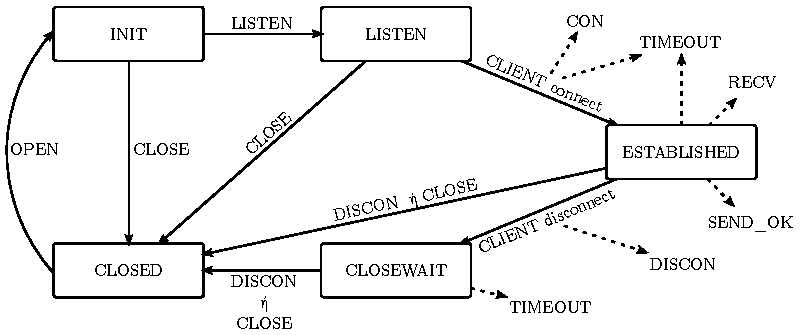
\includegraphics[width=\textwidth]{network_tcp-flow}
    \end{center}
    Βασισμένο. \fullcite[28]{wiz11:w5100:socket-states}
\end{figure}

Στο σχήμα \ref{fig:network:tcp-flow} εμφανίζονται οι βασικές καταστάσεις
(πλαίσια), οι εντολές (συμπαγή βέλη) και τα αίτια πρόκλησης διακοπής (διάστικτα
βέλη) για το Socket του διακομιστή HTTP. Σημειώνεται ότι τα \te{CLIENT connect}
και \te{CLIENT disconnect} αποστέλλονται από τον πελάτη και αποτελούν αιτήματα
έναρξης και λήξης σύνδεσης TCP.

Αρχικά, εφόσον έχει αρχικοποιηθεί το Socket, στέλνοντας την εντολή \te{LISTEN},
το Socket τίθεται σε κατάσταση αναμονής αιτημάτων και παραμένει σε αυτή έως ότου
καταφθάσει αίτημα σύνδεσης. Κατά τη διάρκεια εγκαθίδρυσης της σύνδεσης, το W5100
θέτει το bit CON του καταχωρητή Sn\_IR προκαλλώντας διακοπή (δεδομένου ότι έχουν
ενεργοποιηθεί οι διακοπές για αυτό το Socket) (βλ.
\nameref{ssubsec:network:ir_imr}, σ. \pageref{ssubsec:network:ir_imr}).

Σε κατάσταση ενεργούς σύνδεσης, ο πελάτης στέλνει πακέτα, το φορτίο των οποίων
τοποθετείται στην αφιερωμένη μνήμη εισερχομένων και ενεργοποιείται το bit RECV
του Sn\_IR. Σύμφωνα με το εγχειρίδιο της \textcite[28]{wiz11:w5100}, το RECV
παραμένει ενεργό όσο υπάρχουν διαθέσιμα δεδομένα για ανάγνωση. Τυπικά, η
επεξεργασία των εισερχόμενων δεδομένων προκαλεί την παραγωγή δεδομένων απόκρισης
που τοποθετούνται στην μνήμη εξερχομένων και αποστέλλονται υποβάλλοντας την
εντολή SEND (Sn\_CR). Το bit SEND\_OK (Sn\_IR) ειδοποιεί ότι όλα τα δεδομένα της
μνήμης εξερχομένων έχουν σταλεί. Η διαδικασία ανταλλαγής συνεχίζει για όσο
απαιτείται.

Τελικά, η σύνδεση τερματίζεται είτε ως αποτέλεσμα αιτήματος του πελάτη είτε με
την εντολή \te{DISCON}). Κατόπιν, το Socket αρχικοποιείται και τίθεται, εκ νέου,
σε κατάσταση αναμονής (\te{passive open}).

Στο σχήμα αναφέρεται ένα ακόμα αίτιο διακοπής· η λήξη του χρόνου αναμονής
(\te{TIMEOUT}) κατά την αρχική ή τελική τριπλή χειραψία ή κατά την ανταλλαγή
δεδομένων. Σε κάθε περίπτωση, η αντιμετώπιση του συμβάντος, από πλευράς της
υλοποίησης, είναι, πάντα, ο τερματισμός της σύνδεσης και το κλείσιμο του Socket
ακολουθούμενο από την μετέπειτα επανενεργοποίησή του.

Τυπικά, η υλοποίηση ενδιαφέρεται μόνο για διακοπές που οφείλονται σε εισερχόμενα
δεδομένα, τερματισμό σύνδεσης ή στο πέρας του χρόνου αναμονής. Πάντως,
ανεξαρτήτως περίπτωσης, η ρουτίνα εξυπηρέτησης διακοπών του ακροδέκτη
\nbar{INT}, μεριμνεί για τον καθαρισμό των ενδείξεων που την προκάλεσαν ώστε να
απενεργοποιείται το σήμα του ακροδέκτη μέχρι το επόμενο συμβάν.


\subsection{Low-level API}
%\subsection{Low-level utilities}

Το λογισμικό για την ανταλλαγή δεδομένων μεταξύ μικροελεγκτή και W5100 εργάζεται
με προσωρινούς χώρους αποθήκευσης· μία διεύθυνση στην κύρια μνήμη του
μικροελεγκτή και το πλήθος των Byte που εκτείνονται ξεκινώντας από αυτήν, είναι
αρκετά για την παραλαβή ή αποστολή μερικών Byte. Με διαδοχικές κλήσεις είναι
δυνατό να παραληφθεί ή να αποσταλεί το συνολικό φορτίο. Ωστόσο, στην περίπτωση
του HTTP Socket, τα εισερχόμενα δεδομένα προορίζονται για λεξική ανάλυση,
στοιχειώδους έστω μορφής, ώστε να αναγνωρίζεται η εννοιολογική διάσταση της κάθε
αναπαράστασης.


\subsubsection{Ροή χαρακτήρων}
% SBuffer

Σε αυτήν την περίπτωση, η εργασία με τον οποιοδήποτε προσωρινό χώρο αποθήκευσης
είναι προτιμότερο να αποκρύπτεται από τους αναλυτές, παρέχοντας μία διεπαφή για
τη σειριακή εξαγωγή Byte ή, στην προκειμένη, χαρακτήρων, τον ένα μετά τον άλλο
(ροή χαρακτήρων -- \te{character stream}).
Εναλλακτικά, και χωρίς τήρηση προσωρινού χώρου αποθήκευσης, η διεπαφή μπορεί να
κάνει άμεση χρήση της υποδομής για την ανταλλαγή δεδομένων με το W5100. Ωστόσο,
η τακτική αυτή επιβαρύνει την εξαγωγή κάθε χαρακτήρα με τους υπολογισμούς που
αναφέρονται στην \nameref{ssubsec:network:rx-tx-buffer}
(σ.~\pageref{ssubsec:network:rx-tx-buffer}). Αντιθέτως, προτιμάται η τήρηση
τμημάτων του εισερχόμενου φορτίου σε προσωρινό χώρο, \te{cache}, τοπικά στη
μνήμη του μικροελεγκτή ώστε η οποιαδήποτε επιβάρυνση να υφίσταται μόνο κατά την
ενημέρωση της \te{cache} με την επόμενη ομάδα χαρακτήρων.

Επιπροσθέτως, για την υποστήριξη συμπληρωματικών δυνατοτήτων για την περαιτέρω
διευκόλυνση των αναλυτών, όπως η ανάγνωση κάποιου επόμενου χαρακτήρα (\te{look
forward}) (δηλαδή, χωρίς την υποχρεωτική εξαγωγή όλων των ενδιάμεσων), χωρίς την
υποβάθμιση των επιδόσεών της, η προσωρινή μνήμη υλοποιείται ως δακτύλιος
(κυκλική ουρά). Τα πλεονεκτήματα χρήσης δακτυλίου γίνονται περισσότερο αντιληπτά
λαμβάνοντας υπόψη το σχήμα \ref{fig:network:sbuffer}.

\begin{figure}
    \caption{Ροής χαρακτήρων από τη μνήμη εισερχομένων \te{Socket}.
    \label{fig:network:sbuffer}}
    \begin{center}
    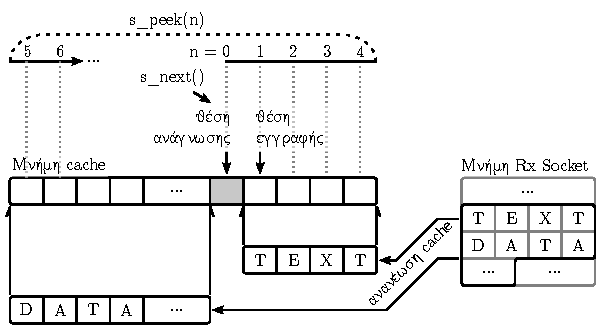
\includegraphics{network_sbuffer}
    \end{center}
\end{figure}

Οι χαρακτήρες τοποθετούνται στη μνήμη \te{cache} σε διαδοχικές θέσεις και
εκτείνονται από τη θέση ανάγνωσης προς το τέλος του αφιερωμένου χώρου μέχρι
(αλλά μη συμπεριλαμβανομένης) τη θέση εγγραφής. Κάθε φορά που εξάγεται ένας
χαρακτήρας από την \te{cache}, η θέση ανάγνωσης αυξάνεται κατά μία θέση ώστε να
προσδιορίζει τον επόμενο για εξαγωγή ή ανάγνωση χαρακτήρα. Αντιστοίχως, όποτε
διαβάζεται μία ομάδα χαρακτήρων από τη μνήμη του \te{Socket}, η θέση εγγραφής
αυξάνεται κατά πλήθος ίσο με αυτό που ελήφθη, ώστε να καταδεικνύεται η επόμενη
της τελευταίας θέσης που ενημερώθηκε με νέο χαρακτήρα. Και οι δύο ενδείξεις
θέσης εκτελούν κυκλική κίνηση, με την έννοια ότι η επόμενη θέση της τελευταίας
διαθέσιμης του αφιερωμένου χώρου είναι πάντα η πρώτη (θέση 0).

Προφανώς, στην περίπτωση κατά την οποία η θέση ανάγνωσης αυξηθεί και ταυτόχρονα
εξισωθεί με τη θέση εγγραφής, η μνήμη \te{cache} έχει εξαντληθεί,
με αποτέλεσμα στην επόμενη χρήση της διεπαφής, να γίνεται προσπάθεια ανάκτησης
της επόμενης ομάδας χαρακτήρων. Το πλήθος των λαμβανόμενων χαρακτήρων εξαρτάται,
σαφώς, από τους εναπομείναντες χαρακτήρες στη μνήμη του Socket και του μη
δεσμευμένου χώρου στην \te{cache} (ο μικρότερος εκ των δύο). Εάν η εξάντληση της
\te{cache} συμβαίνει πάντα στην τελευταία φυσική θέση του αφιερωμένου χώρου, η
χρήση δακτυλίου είναι περιττή.

Ωστόσο, ενδέχεται να προκύψει ανάγκη ανανέωσης πριν την εξάντληση των αποθεμάτων
της \te{cache}. Τέτοιες περιπτώσεις οφείλονται στη χρήση της δυνατότητας
ανάγνωσης (δίχως εξαγωγή), όταν η επιθυμητή θέση βρίσκεται έξω από το
(ενημερωμένο) εύρος της \te{cache}. Όπως στο παράδειγμα του σχήματος
\ref{fig:network:sbuffer}, η ανάγνωση οποιουδήποτε χαρακτήρα έξω από το
ενημερωμένο εύρος (δηλαδή, για $n \ge 1$) προϋποθέτει την ανανέωση της
\te{cache}. Μετά την ολοκλήρωση της πρόωρης ανανέωσης, η θέση εγγραφής
καταλήγει, τις περισσότερες φορές, σε θέση διαφορετική της θέσης 0.
Αυτό ακριβώς το χαρακτηριστικό -- τα ολισθηρά άκρα -- του δακτυλίου εγγυάται τη
συνεχόμενη εισαγωγή και εξαγωγή χαρακτήρων.

Εάν η μνήμη \te{cache} υλοποιηθεί ως (απλή) ουρά, η ανάγκη για πρόωρη ενημέρωση
ενέχει την ενδεχόμενη μετατόπιση των υπαρχόντων χαρακτήρων στις πρώτες θέσεις
του πίνακα ώστε να δημιουργηθεί χώρος για τους νέους χαρακτήρες στο τέλος του
πίνακα. Ωστόσο, κρίνεται ότι αυτή η τακτική είναι λιγότερο αποδοτική και για
αυτόν το λόγο προτιμάται η χρήση δακτυλίου.

Σε κάθε περίπτωση υλοποίησης, η μέγιστη υποστηριζόμενη θέση ανάγνωσης ($n$)
περιορίζεται από το συνολικό μέγεθος της \te{cache} το οποίο καθορίζεται κατά τη
σύνταξη του προγράμματος. Επίσης, στην περίπτωση του δακτυλίου, απαιτούνται το
πολύ δύο αναγνώσεις της μνήμης του Socket για την ενημέρωση της \te{cache}.
Τέλος, σε περίπτωση που τα δεδομένα της μνήμης του Socket έχει εξαντληθεί, όλες
οι συναρτήσεις της διεπαφής επιστρέφουν μία σχετική ένδειξη (EOF).


\subsubsection{Stream match}
\label{ssubsec:network:stream-match}

Μία αναμενόμενη λειτουργία των αναλυτών είναι η επεξεργασία των εισερχόμενων
χαρακτήρων της ροής για την αναγωγή της παρεχόμενης πληροφορίας σε μορφή εύκολα
εκμεταλλεύσιμης από το λογισμικό.

Ο μηχανισμός της υλοποίησης που παρέχεται για αυτόν τον σκοπό βασίζεται στην
παραδοχή ότι κάθε στιγμή που προκύπτει ανάγκη για την αναγνώριση των
εισερχομένων, υπάρχει εκτίμηση σχετικά με το τι αναμένεται να παραληφθεί
(δηλαδή, ποιες είναι οι πιθανές αποδεκτές είσοδοι). Συνεπώς, ένα μέρος της ροής
χαρακτήρων του Socket αντιπαραβάλλεται με ένα προκαθορισμένο σύνολο πιθανών
αλφαριθμητικών. Η επιλογή των «πιθανών» αυτών αλφαριθμητικών γίνεται με γνώμονα
του τι αρμόζει στην κάθε περίπτωση ενεργοποίησης του μηχανισμού.

% \nref: HTTP Parser
Χαρακτηριστική περίπτωση χρήσης του μηχανισμού είναι η ανάλυση ενός αιτήματος
HTTP. Κάθε αίτημα HTTP αρχίζει με τη γραμμή αιτήματος η οποία, το πρώτο πράγμα
που προσδιορίζει είναι η μέθοδος για την επενέργεια στο ακολουθούμενο URI
\parencite[35]{rfc2616}. Το HTTP\slash 1.1 ορίζει οκτώ, συνολικά, μεθόδους, εκ
των οποίων ο διακομιστής μπορεί να τις υποστηρίζει όλες ή ένα υποσύνολό τους.
Όπως είναι αναμενόμενο, κάθε υποστηριζόμενη και, συνεπώς, αναγνωρίσιμη μέθοδος
πρέπει να ορίζεται ως αλφαριθμητικό, ώστε να είναι δυνατή η αντιπαραβολή της με
τους εισερχόμενους χαρακτήρες. Παρότι τα αλφαριθμητικά αποθηκεύονται ανεξάρτητα
το ένα από το άλλο, διατηρείται, ωστόσο, μία συλλογή με αναφορές προς αυτά.
% \nref: σταθερές HTTP Server
Για την απλοποίηση του υποκείμενου μηχανισμού, οι αναφορές τοποθετούνται έτσι
ώστε τα αλφαριθμητικά να εμφανίζονται σε αλφαβητική σειρά και το καθένα
εμφανίζεται μόνο μία φορά.

\begin{figure}
    \caption{Λεξική ανάλυση ροής \te{Socket}. \label{fig:network:stream_match}}
    \begin{center}
    \includegraphics{network_stream_match}
    \end{center}
\end{figure}

Όταν, επομένως, καταφθάνει ένα νέο αίτημα, είναι βέβαιο ότι το πρώτο πράγμα που
πρέπει να προσδιοριστεί είναι η μέθοδος HTTP, με αποτέλεσμα ο μηχανισμός να
ενεργοποιείται με τη συλλογή αλφαριθμητικών των αποδεκτών μεθόδων. Αρχικά,
συμμετέχει ολόκληρο το σύνολο, όπως καθορίζεται από τα όρια \verb~min~ και
\verb~max~ (σχήμα \ref{fig:network:stream_match}).

Η αντιπαραβολή των χαρακτήρων πραγματοποιείται σε επαναλήψεις όπου σε καθεμία,
εξάγεται ένας χαρακτήρας από τη ροή και συγκρίνεται με τον επόμενο χαρακτήρα
των διαθέσιμων αλφαριθμητικών (δηλαδή, των αλφαριθμητικών μεταξύ \verb~min~ και
\verb~max~). Επειδή τα αλφαριθμητικά παρέχονται σε αλφαβητική σειρά, τα όρια
είναι δυνατό να ολισθαίνουν εξαιρώντας όσα αποτυγχάνουν κάποια σύγκριση.

Με τον τρόπο αυτό, τα όρια, σταδιακά, συγκλίνουν προς μία θέση, καταδεικνύοντας
το αλφαριθμητικό που σημειώνει μόνο επιτυχούσες συγκρίσεις. Εφόσον οι
επαναλήψεις τερματιστούν εξαιτίας της εξάντλησης των χαρακτήρων του εν λόγω
αλφαριθμητικού, ενώ έχει εντοπιστεί στη ροή έγκυρος διαχωριστικός χαρακτήρας
(\te{delimiter}) (στην προκειμένη, το κενό διάστημα), η μέθοδος έχει
αναγνωριστεί επιτυχώς. Ένα σημαντικό σημείο είναι ότι, εφόσον ολοκληρωθεί
επιτυχώς η λεξική αναγνώριση, ο εντοπισμένος όρος περιγράφεται αυτομάτως από τη
θέση που κατέχει στην τρέχουσα συλλογή, κάτι που διευκολύνει την αναγγελία του
σε λοιπά μέρη της υλοποίησης, καθώς χρησιμοποιείται κωδικός αριθμός αντί για
αλφαριθμητικό.

Τελικά, η ροή δύναται να υποβληθεί εκ νέου στην ίδια διαδικασία, αυτή τη φορά με
νέα συλλογή αλφαριθμητικών, για παράδειγμα, για την αναγνώριση του αιτούμενου
πόρου.

% εικόνα;


\section{Σύμπλεγμα διακομιστή (HTTP)}
%\section{API διακομιστή (HTTP)}
%\section{Διακομιστής HTTP}

% εικόνα με δομικά στοιχεία συμπλέγματος


\subsection{Κορμός διακομιστή}
% Base
Εφόσον αναγνωριστεί ύπαρξη εισερχόμενων δεδομένων στο Socket του διακομιστή
HTTP, το συμβάν αναγγέλλεται για την εκκίνηση των εργασιών διεκπεραίωσης του.
Από τη βάση του διακομιστή πυροδοτείται ο αναλυτής HTTP για την αναγωγή της
δομής \verb~HTTPRequest~ σύμφωνα με την κεφαλίδα του αιτήματος.
% \nref : (βλ. HTTP Parser).
Η δομή διατηρεί τα βασικά στοιχεία που ενδιαφέρουν το διακομιστή και τις
ρουτίνες περάτωσης για την διεκπεραίωση του αιτήματος
.
%όπως φαίνεται παρακάτω:

%\begin{lstlisting}
%typedef struct HTTPRequest {
%    uint8_t     method;
%    uint8_t     uri;
%    uint8_t     v_major;
%    uint8_t     v_minor;
%    int8_t      accept;
%    uint8_t     transfer_encoding;
%    uint8_t     content_type;
%    uint16_t    content_length;
%    QueryString          query;
%} HTTPRequest;
%\end{lstlisting}

\subsubsection{Γενική συμπεριφορά διακομιστή}

Στην πορεία ελέγχεται η πληρότητα του αιτήματος στο σύνολό του και, σε περίπτωση
κάποιου μη αποδεκτού στοιχείου, επιστρέφονται γενικής φύσεως διαγνωστικά
μηνύματα σφάλματος, όπως στην περίπτωση μη αναγνωρίσιμου URI ή μη διαθέσιμης
μεθόδου. Οι κωδικοί κατάστασης HTTP, αντιστοίχως, είναι 404 (\te{Not Found}) και
405 (\te{Method Not Allowed}), ενώ στην τελευταία περίπτωση συμπεριλαμβάνεται
στην απόκριση το πεδίο κεφαλίδας «Allow» δηλώνοντας τις διαθέσιμες μεθόδους για
το εκάστοτε URI, όπως προτρέπουν οι \textcite[66]{rfc2616}.

Εφόσον τα γενικά χαρακτηριστικά του αιτήματος είναι αποδεκτά, η δομή προωθείται
στην κατάλληλη ρουτίνα περάτωσης, όπως δηλώνεται κατά τη ρύθμιση του διακομιστή.
Οι ρουτίνες περάτωσης είναι ελεύθερες και υποχρεωμένες να παράξουν μία
αρμόζουσα απόκριση HTTP βάσει της παρεχόμενης δομής \verb~HTTPRequest~.
% \nref : (βλ. Ρουτίνες περάτωσης)
Με την ολοκλήρωση της εκτέλεσής τους, ολοκληρώνεται και ο κύκλος του διακομιστή.


\subsubsection{Υποδομή σύνταξης κεφαλίδας}
\label{ssubsec:network:header-compile}

Ένα κοινό χαρακτηριστικό όλων των παραγόμενων αποκρίσεων είναι η ύπαρξη της
κεφαλίδας HTTP. Παρότι τα μηνύματα είναι διαφορετικά σε κάθε περίπτωση, ωστόσο
όλες οι παραγόμενες κεφαλίδες των αποκρίσεων HTTP αποτελούνται, σε μεγάλο βαθμό,
από κοινά πεδία, ενδεχομένως με διαφορετική τιμή. Προκειμένου να εξοικονομείται
χώρος μνήμης που διαφορετικά θα δεσμευόταν για κάθε εμφάνιση πανομοιότυπων
αλφαριθμητικών εντός διαφορετικών μονάδων μεταγλώττισης, παρέχεται μία κεντρική
υποδομή για τη σύνταξη των κεφαλίδων.

Η βασική παραδοχή είναι ότι ένα πλήθος συχνά χρησιμοποιούμενων δομικών
αλφαριθμητικών μονάδων διατηρείται σε μία κεντρική δεξαμενή και παρέχεται ένας
κωδικός αναγνώρισης για την καθεμία. Για τη σύνθεση της επιθυμητής ακολουθίας,
είναι αρκετή η χρήση της διεπαφής παρέχοντας τους αντίστοιχους κωδικούς σε
κατάλληλη σειρά. Εκτός από προκαθορισμένα αλφαριθμητικά, είναι δυνατή η χρήση
ειδικών κωδικών που επιτρέπουν τη συμπερίληψη αυθαίρετων αλφαριθμητικών καθώς
και αριθμών που μετατρέπονται σε κείμενο πριν την αποστολή τους στο Socket
(για την ανταλλαγή δεδομένων Socket, βλ. \nameref{ssubsec:network:rx-tx-buffer}
σ.~\pageref{ssubsec:network:rx-tx-buffer}).

% εικόνα

Για περισσότερη ευχρηστία, η παρεχόμενη διεπαφή πρέπει να είναι ευέλικτη σε
σχέση με το πλήθος των αποδεχόμενων κωδικών. Ο τρόπος με τον οποίο επιτυγχάνεται
είναι ο ορισμός και χρήση συναρτήσεων μεταβλητού πλήθους ορισμάτων (varargs ή
variadic) \parencite{iso:c99}.


\subsubsection{Ανασύνθεση τεμαχισμένων μηνυμάτων}
\label{ssubsec:network:chunked-input}

Το HTTP/1.1 ορίζει μηχανισμό για τη διάσπαση του σώματος ενός μηνύματος σε
τεμάχια καθένα από τα οποία συνοδεύεται από το δικό του αναγνωριστικό μεγέθους,
και επιβάλλεται, στο πλαίσιο του HTTP/1.1, όλες οι υλοποίησεις να υποστηρίζουν
την αποδοχή τέτοιων μηνυμάτων \parencite[25--26]{rfc2616}. Οι βασικοί κανόνες
της δομή του μηνύματος σε αυτήν την περίπτωση, παρουσιάζονται παρακάτω.

\begin{lstlisting}
Chunked-Body   = *chunk
                 last-chunk
                 trailer
                 CRLF
chunk          = chunk-size [ chunk-extension ] CRLF
                 chunk-data CRLF
chunk-size     = 1*HEX
last-chunk     = 1*("0") [ chunk-extension ] CRLF
chunk-data     = chunk-size(OCTET)
trailer        = *(entity-header CRLF)
\end{lstlisting}

Η ύπαρξη τεμαχισμένου σώματος δηλώνεται από το πεδίο κεφαλίδας
«Tranfer-Encoding» με τιμή «\te{chunked}». Σε περίπτωση λήψης ενός αιτήματος με
σχετική ένδειξη, πριν την κλήση της αρμόδιας ρουτίνας περάτωσης, οι αναλυτές
διευθετούνται ώστε να χρησιμοποιούν έναν ελαφρώς διαφορετικό μηχανισμό για την
εξαγωγή χαρακτήρων από τη ροή του Socket, ώστε το σώμα να ανασυντάσσεται στην
αρχική του μορφή χωρίς οι αναλυτές να επιβαρύνονται με τις λεπτομέρειες της
διαδικασίας.

\begin{figure}
    \caption{Μηχανισμός ανασύνθεσης τεμαχισμένου σώματος απόκρισης.
    \label{fig:network:chunked-next}}
    Ο μηχανισμός στηρίζεται και παρέχει συμβατή (ίδια) διεπαφή με το μηχανισμό
    για την εξαγωγή χαρακτήρων από τη ροή
    (\nameref{ssubsec:network:sbuffer} σ.~\pageref{ssubsec:network:sbuffer}).
    \begin{center}
%    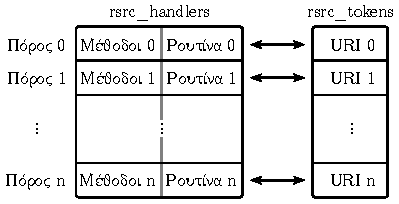
\includegraphics{network_resource-handlers}
    \end{center}
\end{figure}

Όπως παρουσιάζεται στο σχήμα
\ref{fig:network:chunked-next}, ο μηχανισμός ανασύνθεσης (\verb~c_next()~)
βασίζεται στην εξαγωγή χαρακτήρων από τη ροή Socket
(\nameref{ssubsec:network:sbuffer} σ.~\pageref{ssubsec:network:sbuffer}) κυρίως
για την αναγνώριση του μεγέθους κάθε επόμενου τεμαχίου και για την παράλειψη
αυτών των χαρακτήρων από την κανονική ροή. Διαδοχικές χρήσεις της διεπαφής του
μηχανισμού ανασύνθεσης επιστρέφουν το επόμενο Byte, όπως θα συνέβαινε από την
απευθείας χρήση του βασικού μηχανισμού, με τη διαφορά ότι τα εξαγόμενα Byte
καταμετρούνται.

Εφόσον τα Byte ενός τεμαχίου εξαντληθούν (δηλαδή, έχουν αναγνωσθεί τόσα Byte από
τη ροή όσα δηλώθηκαν στο τμήμα \verb~chunk-size~), ο μηχανισμός καταναλώνει τα
Byte που αντιστοιχούν στο μέγεθος του επόμενου τεμαχίου και ο κύκλος
επαναλαμβάνεται. Όταν παραληφθεί το τελευταίο τεμάχιο (μεγέθους 0), ο μηχανισμός
απορρίπτει ενδεχόμενα τερματικά πεδία (\te{trailer}), καθώς, σύμφωνα με τους
\textcite[26]{rfc2616}, ο αποστολέας αποδέχεται ότι τα πεδία του \verb~trailer~
είναι προαιρετικά και μη αναγκαία για την ορθή ερμηνεία του μηνύματος, ενώ στο
πλαίσιο της υλοποίησης κρίνεται μάλλον απίθανη η παραλαβή τεμαχισμένου
μηνύματος, πόσο μάλλον τερματικών πεδίων.


\subsubsection{Παραγωγή τεμαχισμένων μηνυμάτων}
\label{ssubsec:network:chunked-output}

Η υποστήριξη εισερχόμενων τεμαχισμένων μηνυμάτων γίνεται, κυρίως, για λόγους
συμβατότητας με τις προδιαγραφές του πρωτοκόλλου HTTP/1.1. Ωστόσο, η αντίστροφη
διαδικασία -- η παραγωγή αποκρίσεων με τεμαχισμένο σώμα -- κρίνεται ζωτικής
σημασίας ιδίως για την επιστροφή καταχωρημένων μετρήσεων.
% \nref : (βλ. αναγγελία μετρήσεων) [ρουτίνα περάτωσης /measurement]
Ο διακομιστής παρέχει έναν απλό μηχανισμό στις ρουτίνες περάτωσης των αιτημάτων
για τη διατύπωση του μεγέθους κάθε τεμαχίου που πρόκειται να στείλουν. Με τον
τρόπο αυτό, οι ρουτίνες είναι υπεύθυνες μόνο για τη σωστή διάσπαση του σώματος
της απόκρισης σε τμήματα που αυτές μπορούν να χειριστούν.

Όπως έχει αναφερθεί, η υποστήριξη τεμαχισμένων μηνυμάτων είναι υποχρεωτική για
όλες τις υλοποιήσεις HTTP/1.1 όχι, ωστόσο, για αρκετές παλαιότερες υλοποιήσεις
του HTTP/1.0 όπου το πεδίο \te{Transfer-Encoding} είναι άγνωστο
\parencite[25--26,144]{rfc2616}. Στο πλαίσιο της υλοποίησης, η αδυναμία
αποστολής τεμαχισμένου σώματος συνεπάγεται αδυναμία απόκρισης των αντίστοιχων
ρουτινών περάτωσης που κάνουν χρήση του πεδίου.

\subsubsection{Υποδομή σύνταξης κεφαλίδας}


\subsection{Πόροι διακομιστή}

Στον Παγκόσμιο Ιστό, τα URI (\te{Uniform Resource Locator}) -- ακολουθίες
χαρακτήρων δομημένων σύμφωνα με συγκεκριμένους κανόνες σύνταξης --
χρησιμοποιούνται για τον προσδιορισμό αφηρημένων ή φυσικών πόρων, προσβάσιμων
μέσω του Διαδικτύου ή και μη \parencite[1,5]{rfc3986}.
% \nref : Σχετικά με URI parsing.
Στο πλαίσιο της υλοποίησης, τα URI χρησιμοποιούνται για την αναγνώριση των
προθέσεων της αιτούσας οντότητας σε σχέση με τους διαθέσιμους πόρους (ή
υπηρεσίες) της συσκευής. Προκειμένου ο διακομιστής να είναι σε θέση να αποκριθεί
καταλλήλως στα εισερχόμενα αιτήματα, είναι απαραίτητο να γνωρίζει τους
διαθέσιμους πόρους της συσκευής και τις επιτρεπόμενες ενέργειες επί αυτών.
Ιδανικά, η εξέταση και περάτωση κάθε αιτήματος ανατίθεται σε πιο εξειδικευμένα
τμήματα του διακομιστή.
% \nref : Handlers

Συνολικά, τρία είναι τα βασικά στοιχεία που πρέπει να παρέχονται στο διακομιστή
σε ένα πρώτο στάδιο επεξεργασίας των αιτημάτων· το URI, η μέθοδος και, εφόσον
ορίζεται, οι παράμετροι του ερωτήματος (\te{query string}).

\subsubsection{Αναπαράσταση πόρων}

Σχετικά με την πρώτη απαίτηση (γνώση των διαθέσιμων πόρων),
εφόσον τα URI είναι ακολουθίες χαρακτήρων, αρκεί να τηρείται μία συλλογή
αλφαριθμητικών που συγκρίνονται με το URI κάθε αιτήματος ώστε να αποφαίνεται η
αποδοχή ή η απόρριψή του. Στο πλαίσιο της υλοποίησης κρίνεται αρκετή η ύπαρξη
ενός στατικού συνόλου πόρων και, συνεπώς, μίας αντίστοιχης συλλογής.

Σύμφωνα με τους κανόνες σύνταξης της γραμμής αιτήματος ενός HTTP μηνύματος, ο
αναφερόμενος πόρος προσδιορίζεται είτε με πλήρες URI (\verb~absoluteURI~) είτε
με πλήρη διαδρομή (\verb~abs_path~) \parencite[36--37]{rfc2616}.
% \nref : Αναφορά στη σύγκριση με εισερχόμενους χαρακτήρες (stream).
Επιλέγεται να υποστηριχθούν οι πιο κοινές μορφές πλήρων URI και διαδρομών,
σύμφωνα με τους ακόλουθους κανόνες:
\begin{lstlisting}
absoluteURI   = "http:" net_path [ "?" query ]
net_path      = "//" authority [ abs_path ]

abs_path      = "/" segment *( "/" segment )

authority     = host [ ":" port ]
host          = hostname | IPv4address
\end{lstlisting}
Σημειώνεται ότι οι παραπάνω BNF κανόνες αποτελούν μία απλουστευμένη μορφή των
κανόνων σύνταξης όπως αυτοί περιγράφονται από τους \textcite[27--28]{rfc2396}.
Επίσης, θεωρείται ότι ορισμένοι κανόνες (όπως \verb~port~ και 
\verb~IPv4address~) είναι περιττό να αναλυθούν περαιτέρω.

Επομένως, παρατηρείται ότι η διαφορά μεταξύ πλήρους URI και πλήρους διαδρομής
έγκειται στην ύπαρξη του κειμένου \verb~http://~ ακολουθούμενου από το όνομα της
αρχής, στην περίπτωση πλήρους URI. Το κομμάτι της αρχής (\verb~authority~) είναι
δυνατό να αλλάζει (παρότι σχετικά σπάνια) κατά τη λειτουργία της συσκευής, ενώ,
μία δεδομένη στιγμή, είναι ίδια για όλα τα URI. Σε αντίθεση, το \verb~abs_path~
παραμένει σταθερό για κάθε URI. Για τους λόγους αυτούς, κρίνεται προτιμότερη η
συμπερίληψη μόνο του τμήματος \verb~abs_path~ στα αλφαριθμητικά της συλλογής,
και η εφαρμογή ξεχωριστών επιπρόσθετων ελέγχων σε περίπτωση που παρέχεται πλήρες
URI.

Κάθε πόρος δύναται να υποστηρίζει διαφορετικές μεθόδους και, επομένως, οι
διαθέσιμες μέθοδοι πρέπει να προσδιορίζονται για τον καθένα ξεχωριστά. Το ίδιο
ισχύει και για τις παραμέτρους ερωτήματος. Ωστόσο, σε αντίθεση με τις μεθόδους,
οι παράμετροι έχουν την ιδιαιτερότητα ότι η επιλογή τους γίνεται αυθαίρετα και
όχι από ένα σαφώς προσδιορισμένο σύνολο, όπως στην περίπτωση των μεθόδων. Ο
τρόπος υποστήριξης παραμέτρων ερωτήματος αναλύονται στη σελίδα
\pageref{ssubsec:network:query-string}.
Επίσης, αναφέρθηκε ότι η ρουτίνα εξυπηρέτησης των αιτημάτων κάθε πόρου είναι
καλύτερο να αποτελεί μία ξεχωριστή διακριτή οντότητα. Συνεπώς, κρίνεται χρήσιμος
ο ορισμός μίας δομής η οποία παρέχει την πληροφορία URI-μέθοδοι-ρουτίνα για κάθε
πόρο.

Ωστόσο, προκειμένου η συλλογή αλφαριθμητικών να είναι συμβατή με την υποδομή
\verb~stream_match()~, τα αλφαριθμητικά πρέπει να αποθηκεύονται σε διαδοχικές
θέσεις μνήμης, κάτι που ο ορισμός του αλφαριθμητικού εντός της δομής, αποτρέπει.
Επομένως, προτιμάται, αρχικά, ο ορισμός της ακόλουθης δομής για την μερική
περιγραφή ενός πόρου:
\begin{lstlisting}
typedef struct ResourceHandler {
    uint8_t methods;
    void (*call)(struct HTTPRequest*);
} ResourceHandler;
\end{lstlisting}
Τυπικά, διατίθεται ένα σύνολο πόρων (και όχι μόνο ένας) και, συνεπώς, απαιτείται
μία συλλογή τέτοιων δομών και μία ακόμα συλλογή με τα αντίστοιχα URI. Η σύνδεση
μεταξύ τους γίνεται βάσει της θέσης που κατέχει η κάθε δομή και το URI μέσα στις
αντίστοιχες συλλογές, όπως περιγράφεται και στο σχήμα
\ref{fig:network:resource-handlers}.

\begin{figure}
    \caption{Περιγραφή πόρων διακομιστή.
    \label{fig:network:resource-handlers}}
    Κάθε πόρος περιγράφεται στο διακομιστή HTTP από ένα URI, τις αποδεκτές HTTP
    μεθόδους και μία αφιερωμένη ρουτίνα περάτωσης του αιτήματος.
    \begin{center}
    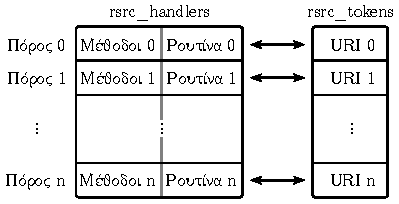
\includegraphics{network_resource-handlers}
    \end{center}
\end{figure}


\subsubsection{Παράμετροι ερωτήματος}
\label{ssubsec:network:query-string}

Όπως αναφέρουν οι \textcite[23--24]{rfc3986} για τις προδιαγραφές του URI, ως
ερώτημα (\te{query}) ορίζονται μη ιεραρχικά δεδομένα που συνοδεύουν το τμήμα της
διαδρομής του URI, η έναρξη των οποίων σηματοδοτείται από το χαρακτήρα «?», και
η λήξη, από τον «\#» ή, εναλλακτικά, το τέλος του URI, με συνηθισμένη σύνταξη
για τη δήλωσή τους, ζεύγη της μορφής «παράμετρος=τιμή». Στο πλαίσιο της
υλοποίησης, κρίνεται σκόπιμη η υποστήριξη τους, κατά κύριο λόγο, για την παροχή
της αιτούσας οντότητας ενός μηχανισμού για τον έλεγχο των αποτελεσμάτων
αναζήτησης.
% \nref: /measurement handler. Μία τέτοια περίπτωση εφαρμογής αναφέρεται στην

Τα ερωτήματα έχουν την ιδιαιτερότητα όχι χαρακτηρίζονται από μεγάλη
ποικιλομορφία· για κάθε URI είναι δυνατό να υποστηρίζονται αυθαίρετα επιλεγμένα
αλφαριθμητικά ως παράμετροι και αντίστοιχων τιμών. Στο πλαίσιο της υλοποίησης,
ενδιαφέρει η ύπαρξη μίας υποδομής για την αναγνώριση μόνο εκείνων των παραμέτρων
ερωτήματος των εισερχόμενων αιτημάτων που ορίζονται και έχουν νόημα για το
εκάστοτε URI, ενώ παράλληλα, παρέχεται ένας χώρος για τη διατήρηση των δοθέντων
τιμών με σκοπό τη μετέπειτα επεξεργασία τους από τις αρμόδιες ρουτίνες.

Για το σκοπό αυτό ορίζεται η δομή \verb~QueryString~ (σχήμα
\ref{{fig:network:query-string}}) όπου κεντρικού ενδιαφέροντος είναι τα μέλη
\verb~tokens~, \verb~values~ και \verb~buff~. Σε ένα πρώτο στάδιο του κύκλου
ζωής της δομής, η συλλογή \verb~tokens~ συμπληρώνεται με τις αποδεκτές
παραμέτρους του τρέχοντος URI (κατόπιν αναγνώρισής του), ενώ τα στοιχεία της
\verb~values~ αρχικοποιούνται σε NULL υποδηλώνοντας ότι η τιμή όλων των
παραμέτρων είναι αόριστη.

Κατά τη διάρκεια ανάλυσης του υπολειπόμενου URI, οι εισερχόμενοι χαρακτήρες
συγκρίνονται με τις διαθέσιμες παραμέτρους (εφόσον υπάρχουν), προκειμένου να
εντοπιστεί κάποιο ταίριασμα, στην οποία περίπτωση οι εισερχόμενοι χαρακτήρες που
αντιστοιχούν στην τιμή (δηλαδή, μετά το =), αντιγράφονται στο χώρο \verb~buff~
και ενημερώνεται ακολούθως η συλλογή \verb~values~ ώστε να καταδεικνύεται το
αντίστοιχο αλφαριθμητικό της εντοπισμένης παραμέτρου.

Με το πέρας της ανάλυσης του URI, κάθε στοιχείο της συλλογής \verb~values~
είτε έχει παραμείνει NULL είτε διαθέτει αναφορά σε κάποια θέση του \verb~buff~
από την οποία εκτείνεται ένα αλφαριθμητικό (τερματισμένο με το χαρακτήρα NULL).
Η σημασιολογική, πλέον, ανάλυση των τιμών ανατίθεται είναι δυνατό να ανατεθεί
στην αντίστοιχη ρουτίνα περάτωσης τους αιτήματος μετά την ολοκλήρωση της
ανάλυσης και του υπόλοιπου αιτήματος.

\begin{figure}
    \caption{Δομή αναπαράστασης ερωτήματος URI.
    \label{fig:network:query-string}}
    \begin{center}
    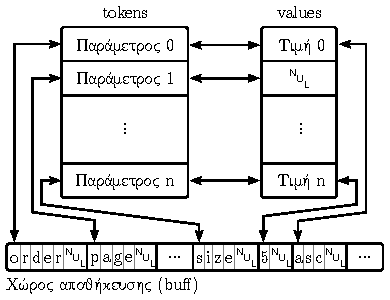
\includegraphics{network_query-string}
    \end{center}
\end{figure}
















